\section{DC}

\begin{frame}{Round Reduced Attack}
\begin{figure}[H]
        \centering
        \minipage{\textwidth}
        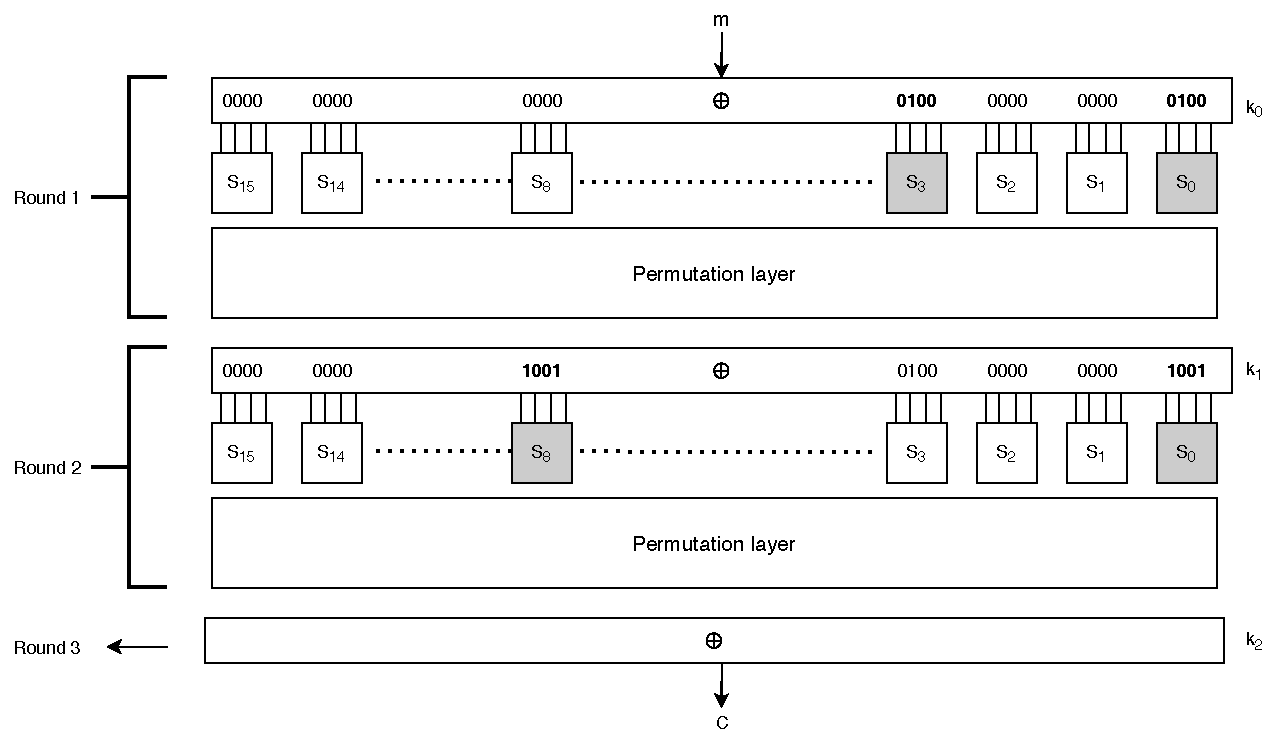
\includegraphics[width=\linewidth]{DC1.pdf}
        \endminipage
        \caption{Attack Model}
    \end{figure}
\end{frame}


\begin{frame}{The Difference Distribution Table}
\begin{figure}[h!]
    \centering
    \scalebox{0.8}{
    \begin{tabular}{ |c||c|c|c|c|c|c|c|c|c|c|c|c|c|c|c|c| }
        \hline
         & 0 & 1 & 2 & 3&4& 5& 6&7&8&9&A&B&C&D&E&F  \\ \hline \hline
         0& 16 & 0 & 0 & 0 &0 &0 &0 &0& 0& 0 &0& 0& 0 &0& 0& 0 \\ 
         1& 0 & 0 & 0 & 4 & 0 & 0 & 0 & 4 & 0 & 4 &0& 0& 0 &4& 0& 0 \\
         2& 0 & 0 & 0 & 2 & 0 & 4 & 2 & 0 & 0 & 0 &2& 0& 2 &2& 2& 0 \\
         3& 0 & 2 & 0 & 2 & 2 & 0 & 4 & 2 & 0 & 0 &2& 2& 0 &0& 0& 0 \\
         4& 0 & 0 & 0 & 0 & 0 & 4 & 2 & 2 & 0 & 2 &2& 0& 2 &0& 2& 0 \\
         5& 0 & 2 & 0 & 0 & 2 & 0 & 0 & 0 & 0 & 2 &2& 2& 4 &2& 0& 0 \\
         6& 0 & 0 & 2 & 0 & 0 & 0 & 2 & 0 & 2 & 0 &0& 4& 2 &0& 0& 4 \\
         7& 0 & 4 & 2 & 0 & 0 & 0 & 2 & 0 & 2 & 0 & 0 & 0 & 2 & 0 & 0 & 4\\
         
         8& 0 & 0 & 0 & 2 & 0 & 0 & 0 & 2 & 0 & 2 & 0 & 4 & 0 & 2 & 0 & 4\\
         9& 0 & 0 & 2 & 0 & 4 & 0 & 2 & 0 & 2 & 0 & 0 & 0 & 2 & 0 & 4 & 0\\
         A& 0 & 0 & 2 & 2 & 0 & 4 & 0 & 0 & 2 & 0 & 2 & 0 & 0 & 2 & 2 & 0\\
         B& 0 & 2 & 0 & 0 & 2 & 0 & 0 & 0 & 4 & 2 & 2 & 2 & 0 & 2 & 0 & 0\\
         C& 0 & 0 & 2 & 0 & 0 & 4 & 0 & 2 & 2 & 2 & 2 & 0 & 0 & 0 & 2 & 0\\
         D& 0 & 2 & 4 & 2 & 2 & 0 & 0 & 2 & 0 & 0 & 2 & 2 & 0 & 0 & 0 & 0\\
         E& 0 & 0 & 2 & 2 & 0 & 0 & 2 & 2 & 2 & 2 & 0 & 0 & 2 & 2 & 0 & 0\\
         F& 0 & 4 & 0 & 0 & 4 & 0 & 0 & 0 & 0 & 0 & 0 & 0 & 0 & 0 & 4 & 4\\ \hline
    \end{tabular}
    }
    \captionof{table}{DDT of the S-box}\label{fig2}
\end{figure}
\end{frame}


\begin{frame}{Differential Characteristics}
\begin{figure}[h!]
        \centering
        \begin{tabular}{ |c||c|c|c| }
            \hline
             Rounds & & Diff. & Prob. \\ \hline \hline
             I& & $x_0 = 4$, $x_4 = 4$ &  \\ 
             $R_1$& $k_0$ & $x_0 = 4$, $x_4 = 4$ & 1 \\
             $R_1$& S & $x_0 = 5$, $x_{3} = 5$ & $2^{-4}$ \\
             $R_1$& P & $x_0 = 9$, $x_{8} = 9$ & 1 \\
             $R_2$& $k_1$ & $x_0 = 9$, $x_{8} = 9$ & 1 \\ \hline
        \end{tabular}
        \captionof{table}{Characteristics}\label{fig7}
    \end{figure}
    \begin{block}{Characteristic}
        ($x_0 = 4$, $x_3 = 4$) $\xrightarrow[]{\text{R}}$ ($x_0 = 9$, $x_8 = 9$)
    \end{block}
\end{frame}

\begin{frame}{Idea of filtering}
    \begin{itemize}
        \item Decrease Wrong pair $\xrightarrow[]{}$ Idea of filtering
        \item Observe from the DDT that transitions from $9 \xrightarrow[]{} \{2,4,6,8,c,e\}$
        \item Thus, after the effect of permutation layer of the second round, $c_1 \oplus c_2$ must belong to the set given below : \\ 
        $\{\{x_4=1,x_6=1\},\{x_6=1,x_8=1\},\{x_4=1,x_6=1,x_8=1\},\{x_6=1,x_{12}=1\},\{x_6=1,x_8=1,x_{12}=1\},...\}$ We have written code for this.
    \end{itemize}
    \begin{block}{Filtering}
        Thus, message pair leading to the cipher text difference other than the above set, can be discarded. 
    \end{block}
\end{frame}

\begin{frame}{Key Guess}
    \begin{figure}[H]
        \centering
        \minipage{\textwidth}
        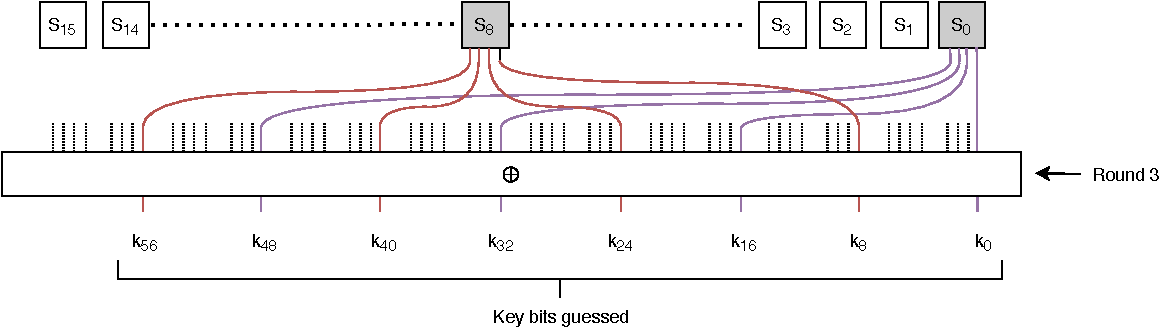
\includegraphics[width=\linewidth]{DC2.pdf}
        \endminipage
        \caption{Attack Model}
    \end{figure}
    \begin{itemize}
        \item Guess 8 bits of the key $k_2$ as shown in the figure.
        \item The probability that the result of partial decryption probabilistically matches $\Delta$out is $<<1$.
        \item Thus, the right guess reaches $\Delta$out more than any other
wrong guess
    \end{itemize}
\end{frame}